\documentclass[11pt,aspectratio=169,reqno]{beamer}

\usepackage[labelformat=empty]{caption}
\usepackage[version=4]{mhchem}

\usepackage{tikz}
\usetikzlibrary{arrows.meta}

\usepackage{biblatex}
\addbibresource{../sources.bib}

\title{Lösungen einfacher Differentialgleichungssysteme zur Autoregulation}
\date[28.03.2023]{28.03.2023}
\author{Mario Kunz, Xaver Hanushevsky}
\institute{D-BIOL}

\usetheme{eth}

\colorlet{titlefgcolor}{ETHBlue}
\colorlet{accentcolor}{ETHRed}

\newcommand{\highlightpause}{\addtocounter{beamerpauses}{-1}\pause\color<+>{ETHPurple}}

\begin{document}

\setlength{\titleboxwidth}{0.65\textwidth}
\titleframe

% Wer die bessere Idee hat
\begin{frame}[fragile]{Intro}
    Etwas Kreatives einfallen lassen für hier
\end{frame}

% Xaver
% shorten?
\begin{frame}{Das Lac Operon}
\begin{columns}
    \column{.4\textwidth}

    \begin{itemize}
        \item Positive Regulation durch cAMP\\
        \begin{itemize}
            \item cAMP Synthese inhibiert in Präsenz von \emph{Glucose}
            \item cAMP bindet and CRP
            \item Homodimer bindet vor Promoter an DNA
            \item Interaktion mit $\alpha$-Untereinheit von RNA Pol führt zu Initiation
        \end{itemize}
        \item Negative Regulation durch freies LacI-Protein
        \begin{itemize}
            \item Allolactose inaktiviert LacI \\ $\ce{Lactose $\xrightleftharpoons{LacY}$ Allolactose}$
        \end{itemize}
        \item[$\Rightarrow$] Lac Operon nur exprimiert in Präsenz von Lactose und Abwesenheit von Glucose
    \end{itemize}

    {\tiny cAMP = cyclic AMP, CRP = cAMP receptor protein}
    
    \column{.6\textwidth}
    \begin{figure}
        \centering
        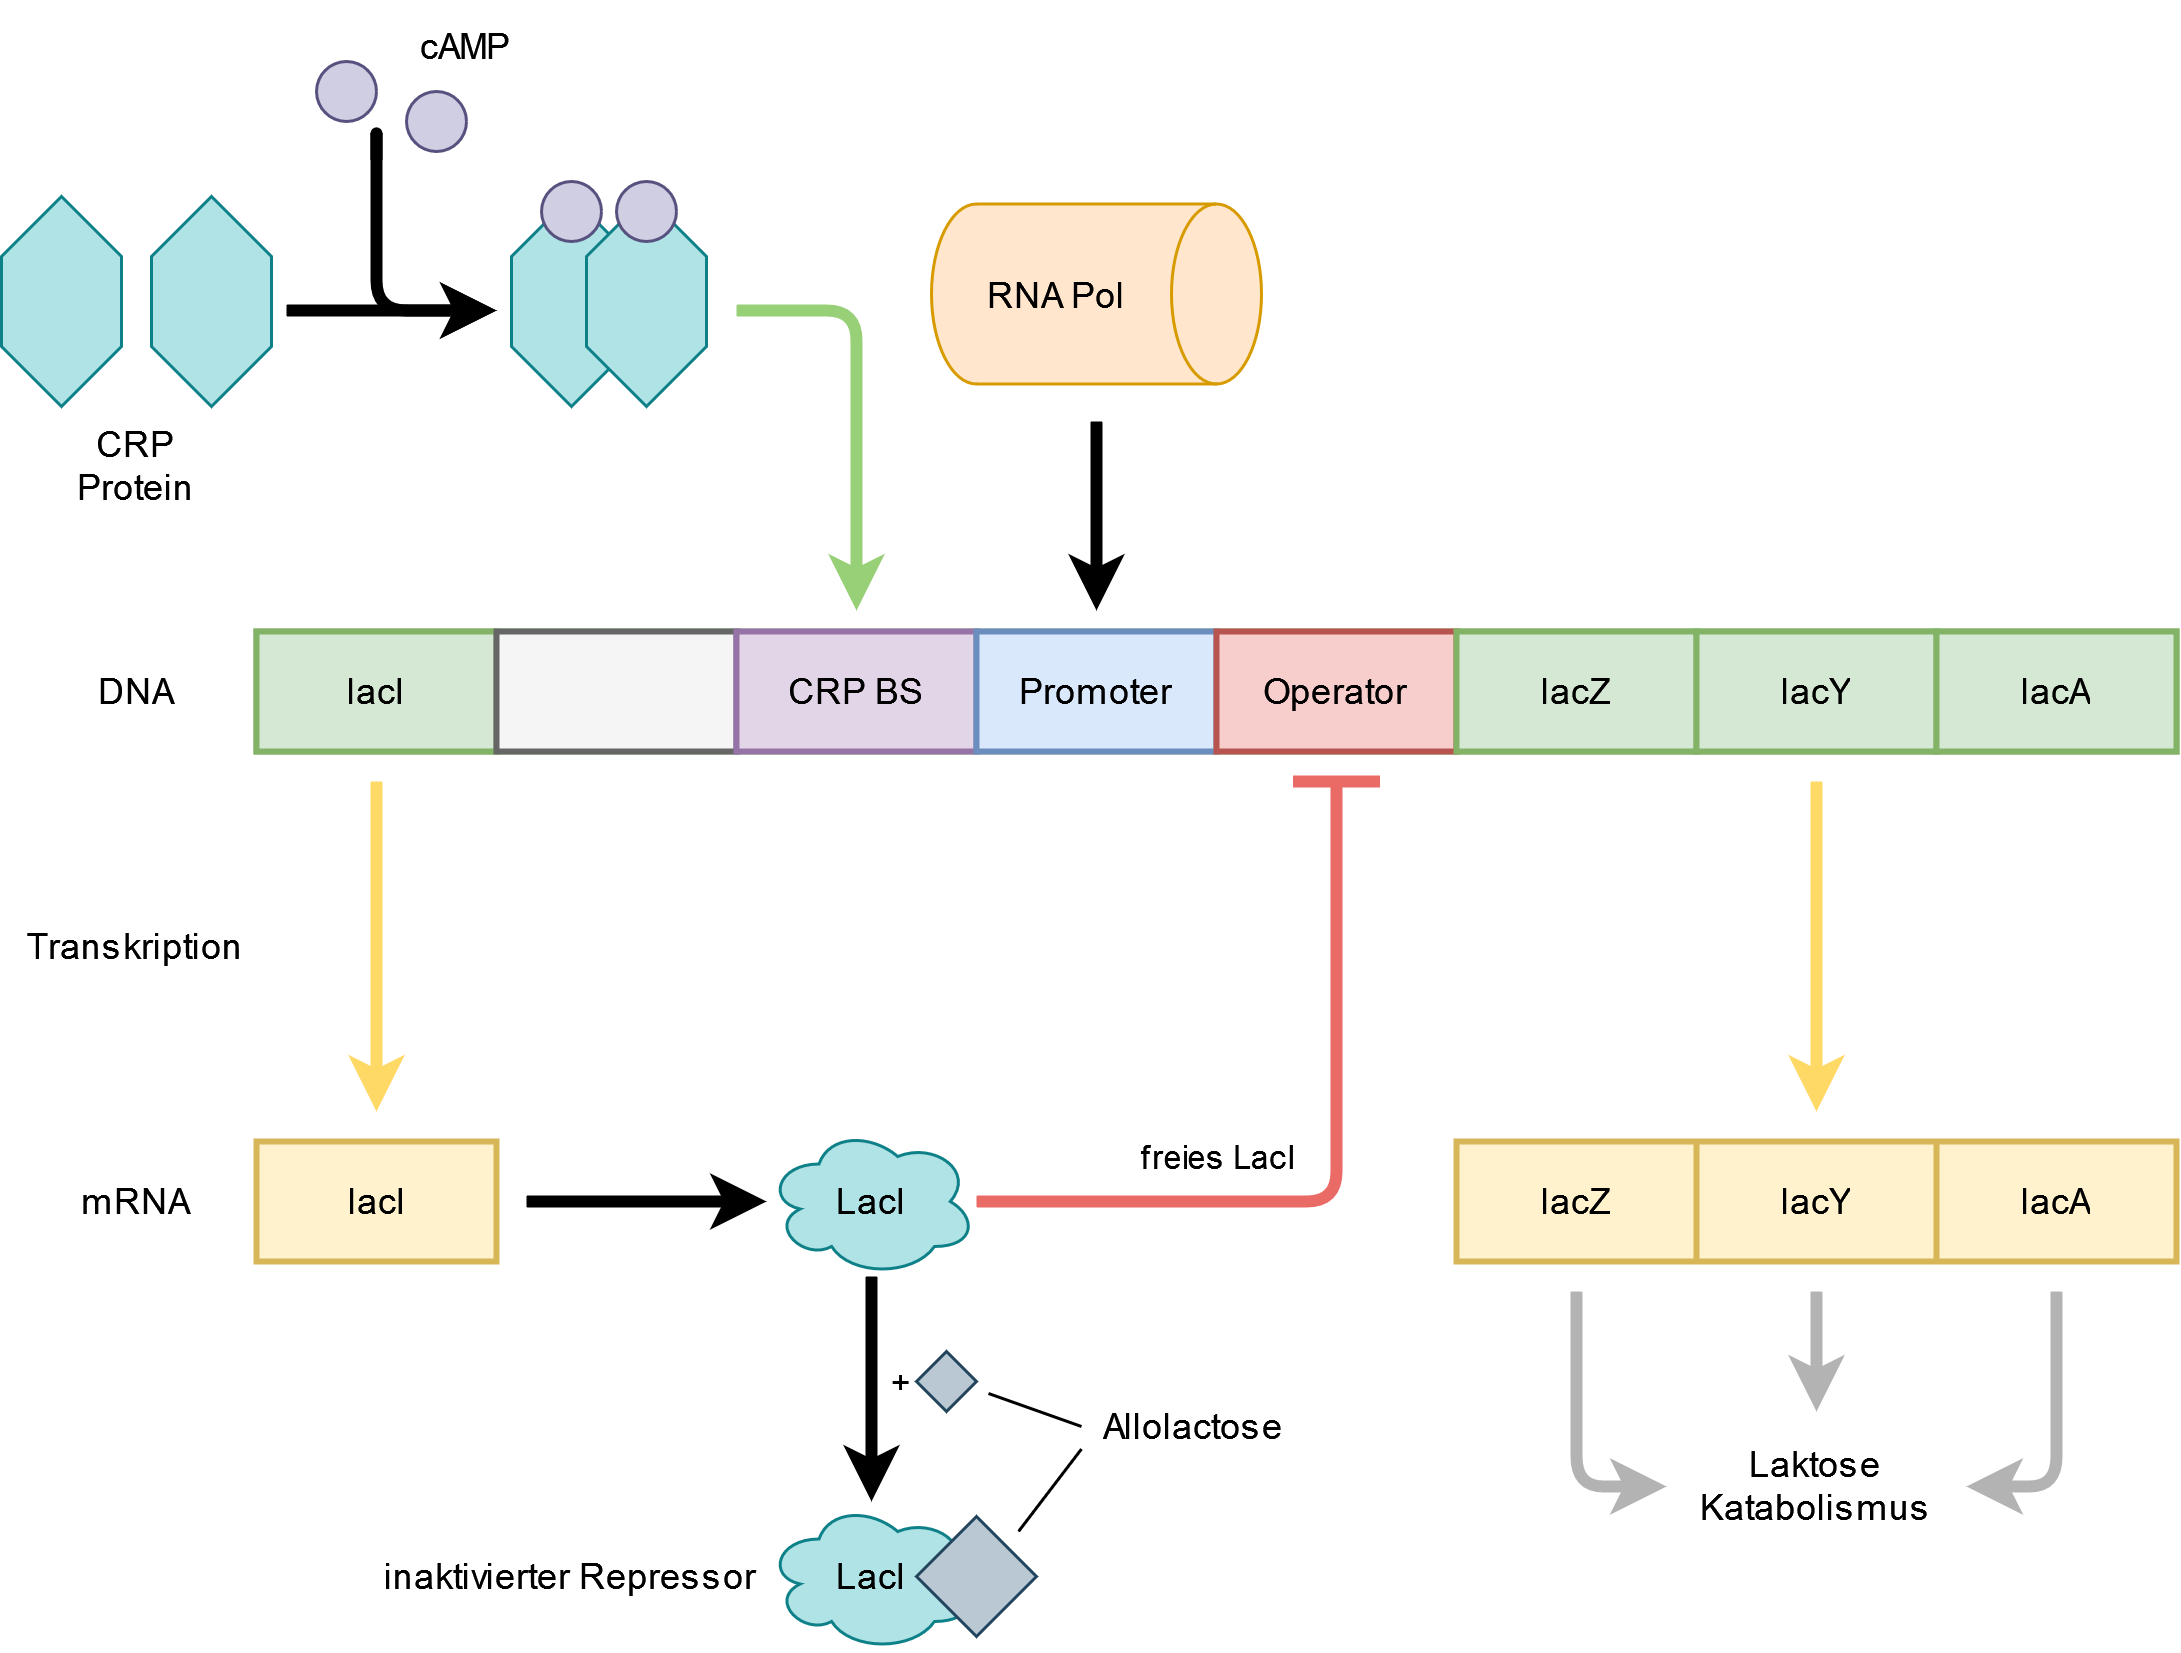
\includegraphics[width=\textwidth]{images/lac_operon.png}
    \end{figure}
\end{columns}
\end{frame}

% Xaver
\begin{frame}{Rückkopplung im Kontext der Genexpression}
\begin{columns}
    \column{.5\textwidth}
    \centering
    \textbf{Positive Rückkopplung}
    \begin{figure}
        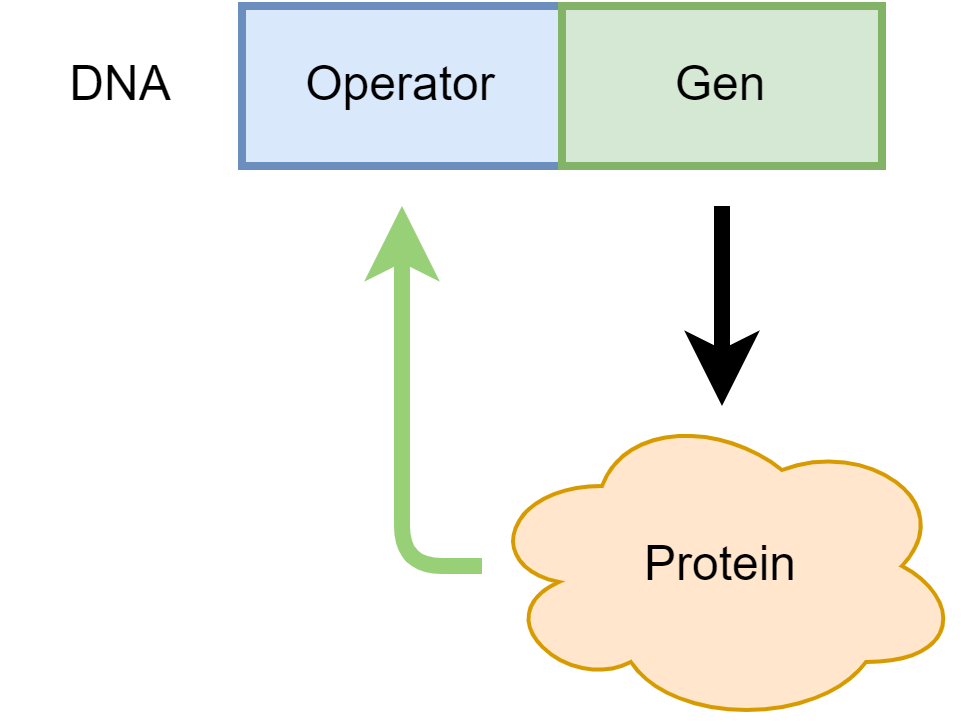
\includegraphics[width=.6\textwidth]{images/dna_positive_autoregulation.png}
    \end{figure}

    Gebundenes Protein führt zu Rekrutierung von RNA Polymerase\\[1em]
    mehr Protein $\Rightarrow$ \textbf{mehr} Protein
    \vspace{1em}

    \uncover<2->{
        \begin{tabular}{l | l}
            initiale Konzentration = 0 & nie Protein \\
            \hline
            Verhalten gegen $t=\infty$ & intuitiv $[\text{P}]=\infty$
        \end{tabular}
    }
    \only<3>{
        \begin{tikzpicture}[remember picture,overlay]
            \node[xshift=0.8cm, yshift=-4cm] at (current page.center) {\textcolor{ETHRed}{macht das Sinn?}};
            \draw[ETHRed, line width=1pt, arrows = {-Stealth[length=8pt, inset=2pt]}] (0,-0.8) -- (-0.7,-0.4);
        \end{tikzpicture}
    }
    
    \column{.5\textwidth}
    \centering
    \textbf{Negative Rückkopplung}
    \begin{figure}
        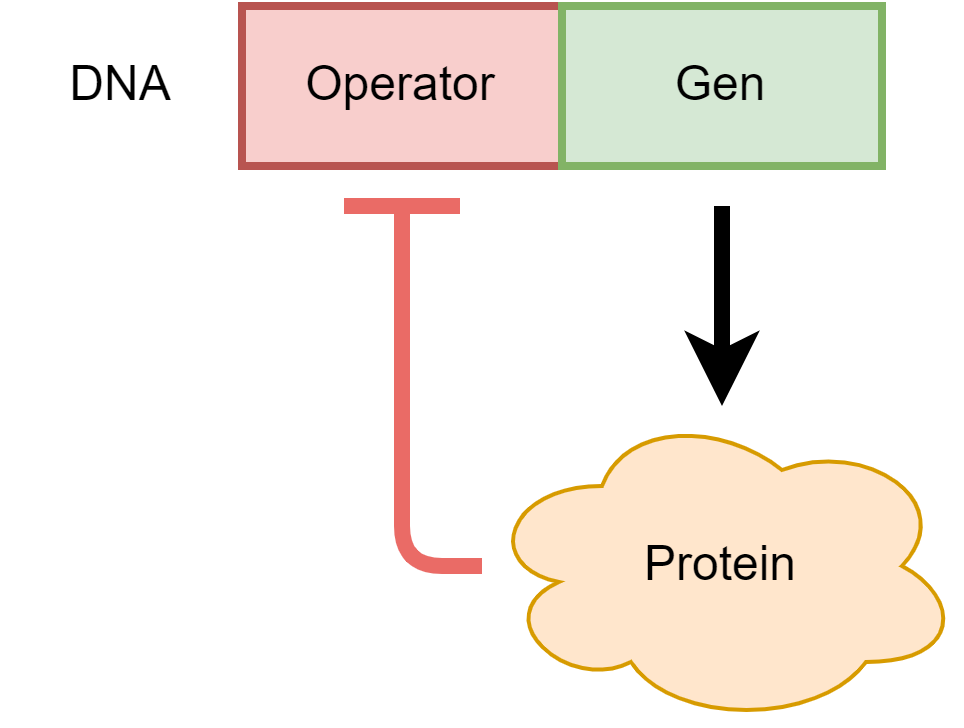
\includegraphics[width=.6\textwidth]{images/dna_negative_autoregulation.png}
    \end{figure}
    Freier Operator erlaubt Transkription\\[2em]
    mehr Protein $\Rightarrow$ \textbf{weniger} Protein
    \vspace{1em}

    \uncover<4->{
        \begin{tabular}{ l | l }
            initiale Konzentration = 0 & sofortige Ausprägung \\
            \hline
            Verhalten gegen $t=\infty$ & ?
        \end{tabular}
    }
    
\end{columns}
\end{frame}

% Mario
\begin{frame}{Ziel unserer Arbeit}
\begin{columns}
    \column{.5\textwidth}

    \begin{itemize}
        \item Mathematisches Modell für
        \begin{enumerate}
            \item negative Autoregulation
            \item positive Autoregulation
        \end{enumerate}
        \item mRNA- und Protein-Konzentration soll beachtet werden
        \begin{itemize}
            \item Verhältnis mRNA:Protein untersuchbar
        \end{itemize}
        \item numerische Lösung mit MATLAB
        \begin{itemize}
            \item \emph{da die Systeme nicht analytisch lösbar sein werden}
        \end{itemize}
    \end{itemize}
    
    \column{.5\textwidth}
    \begin{figure}
        \centering
        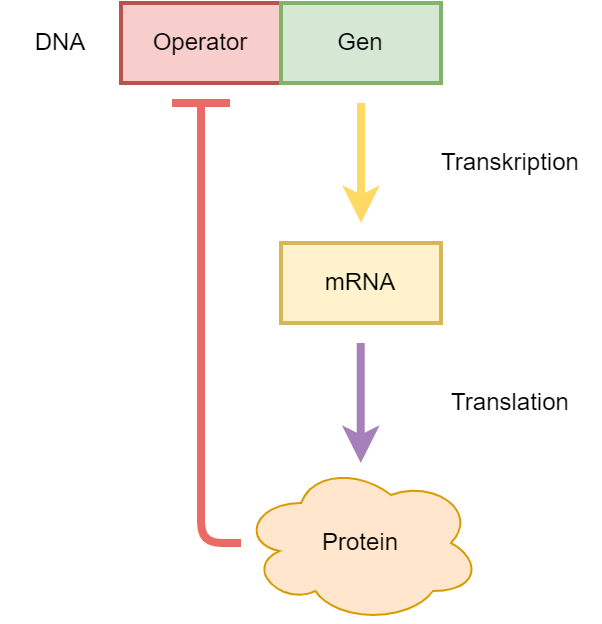
\includegraphics[width=.7\textwidth]{images/repression.png}
        \caption{\tiny Negative Autoregulation}
    \end{figure}
\end{columns}
\end{frame}

% Mario
\begin{frame}{Negative Autoregulation über mRNA und Repressorprotein}
    \centering Nur freie DNA führt zu Transkription\\[1em]
    mehr Protein $\Rightarrow$ \textbf{weniger} freie DNA $\Rightarrow$ \textbf{weniger} Transkription $\Rightarrow$ \textbf{weniger} Protein

    \vspace{2em}

    \begin{figure}
        \centering
        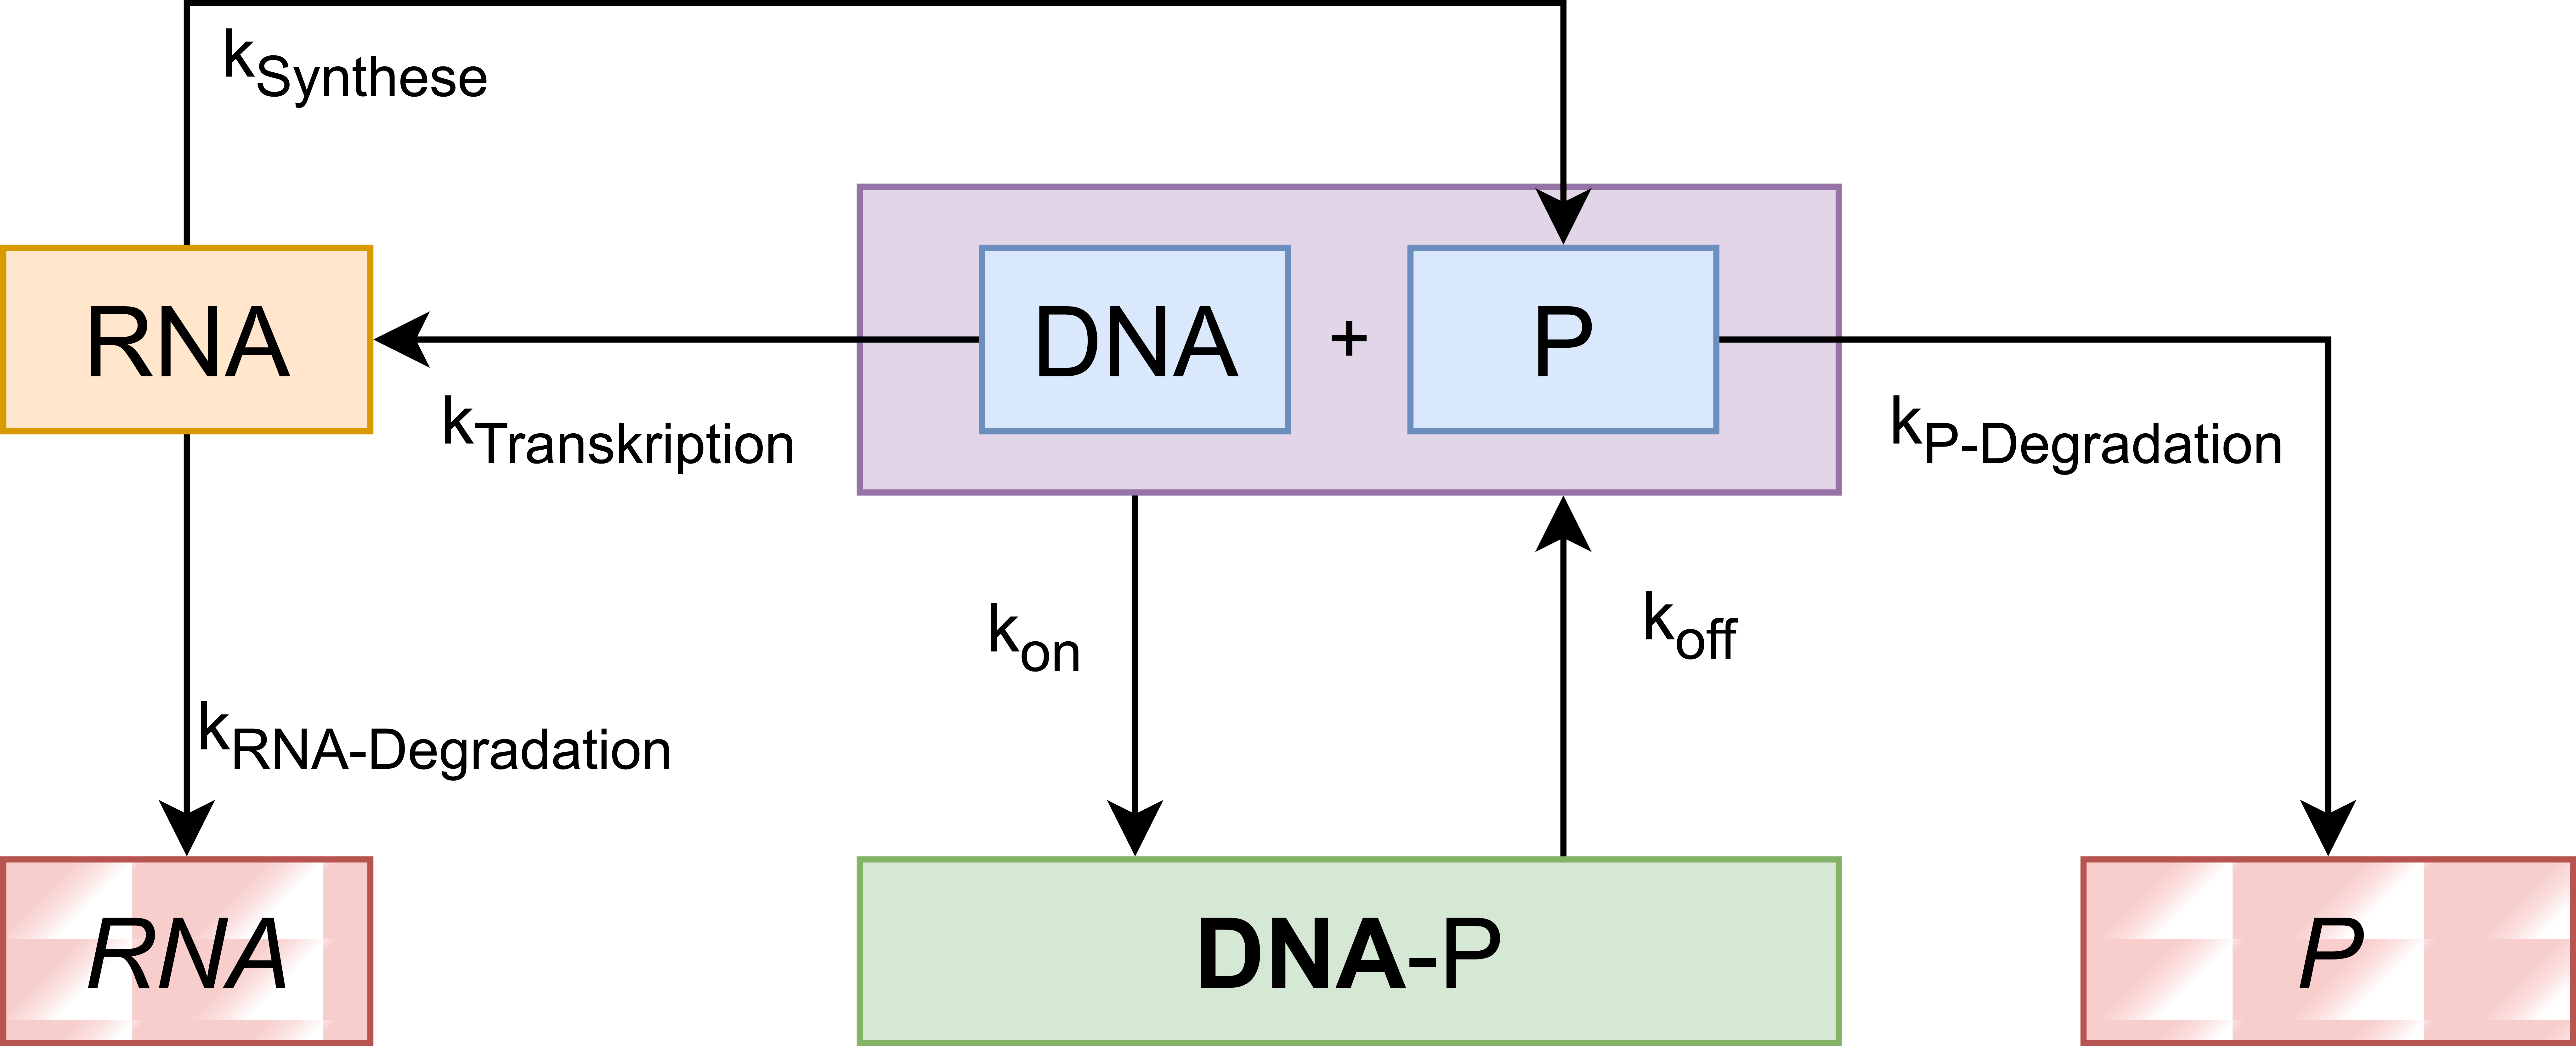
\includegraphics[width=.6\textwidth]{images/negative_autoregulation_overview.png}
    \end{figure}
\end{frame}

% Mario
\begin{frame}{Gleichgewicht zwischen gebundener und freier DNA}
    \begin{tikzpicture}[remember picture,overlay]
        \node[xshift=-2cm,yshift=-1.5cm] at (current page.north east) {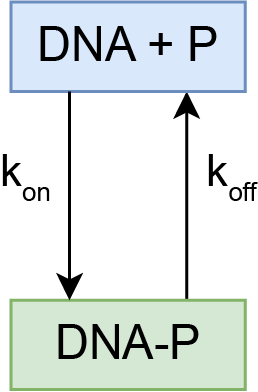
\includegraphics[width=2cm]{images/DNA-binding_equilibrium.png}};
    \end{tikzpicture}

    Hin- und Rückreaktionen im Gleichgewicht
    \begin{itemize}
        \item $v_\text{on}=k_\text{on}\cdot [\text{DNA}]\cdot [\text{P}]$
        \item $v_\text{off}=k_\text{off}\cdot [\text{DNA-P}]$\pause
    \end{itemize}

    \vspace{1.5em}

    \begin{columns}[onlytextwidth]
    \column{.4\textwidth}
    Für die folgenden Schritte nehmen wir an, dass sich das DNA-Protein Gleichgewicht sehr schnell einstellt, denn dann gilt:
    \column{.6\textwidth}
    \begin{itemize}
        \item $v_\text{on}=v_\text{off}$\\[8pt]
        \item $\dfrac{d[\text{DNA}]}{dt}=-\dfrac{d[\text{DNA-P}]}{dt}=0$\\[8pt]
    \end{itemize}
    \[k_\text{on}\cdot [\text{DNA}]\cdot [\text{P}]=k_\text{off}\cdot [\text{DNA-P}]\]
    \end{columns}
\end{frame}

% Mario
\begin{frame}{Gleichgewicht zwischen gebundener und freier DNA}
    \begin{columns}[T]
    \column{.3\textwidth}
    \centering
    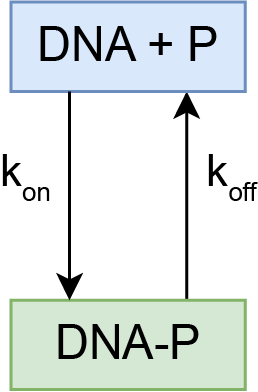
\includegraphics[width=2cm]{images/DNA-binding_equilibrium.png}
    \column{.3\textwidth}
    \[K=\frac{k_\text{off}}{k_\text{on}}=\frac{[\text{DNA}]\cdot [\text{P}]}{[\text{DNA-P}]}\]\pause
    \column{.3\textwidth}
        \[[\text{DNA$_\text{Total}$}]=[\text{DNA}]+[\text{DNA-P}]\]\\[-2em]
        \[[\text{DNA}]=[\text{DNA$_\text{Total}$}]-[\text{DNA-P}]\]
    \end{columns}

    \vspace{4em}
    \highlightpause
    
    \parbox{\textwidth}{
    % \[\Downarrow\]
    % \[K=\frac{([\text{DNA$_\text{Total}$}]-[\text{DNA-P}])\cdot [\text{P}]}{[\text{DNA-P}]}\]\\
    % \[K\cdot[\text{DNA-P}]=[\text{DNA$_\text{Total}$}]\cdot [\text{P}]-[\text{DNA-P}]\cdot [\text{P}]\]
    % \[[\text{DNA-P}]\cdot(K+[\text{P}])=[\text{DNA$_\text{Total}$}]\cdot [\text{P}]\]\\
    \[[\text{DNA-P}]=\frac{[\text{DNA$_\text{Total}$}]\cdot [\text{P}]}{K+[\text{P}]}\]
    }
\end{frame}

% Mario
\begin{frame}{Vergleich mit Bindungsgleichgewichte, Grundlagen der Biologie 1}
    \begin{columns}
        \column{.4\textwidth}
        Konzentration der besetzten DNA\vspace{1em}
        \[[\text{DNA-P}]=[\text{DNA$_\text{Total}$}]\cdot\color{ETHPurple}\frac{[\text{P}]}{K+[\text{P}]}\]
        \pause
        
        \column{.6\textwidth}
        \begin{figure}
            \centering
            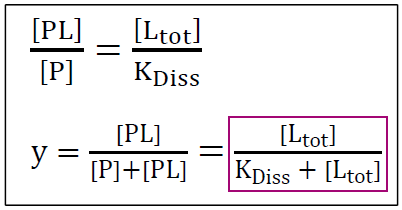
\includegraphics[width=.6\textwidth]{images/occuption_degree_glockshuber.png}
            \caption*{\tiny Skript Prof. Dr. Rudolf Glockshuber, S. 32}
        \end{figure}
        
        \begin{description}
            \item[$K_\text{Diss}$] Dissoziationskonstante der Protein-Ligand-Paares
            \item[$\lbrack L_\text{tot}\rbrack$] Totale Konzentration des Liganden
            \item[$y$] Besetzungsgrad des Proteins
            \item[$K_\text{Diss}=\lbrack L_\text{tot}\rbrack$] 50\% des Proteins sind besetzt
        \end{description}
    \end{columns}
\end{frame}


% Mario
\begin{frame}{Vom Besetzungsgrad zum Nichtbesetzungsgrad}
\begin{block}{Negative Autoregulation}
    RNA wird \textbf{nur} transkribiert, wenn die DNA \textbf{nicht} besetzt ist
\end{block}

\begin{align*}
    z&=1-\frac{[\text{P}]}{K+[\text{P}]}\\[2em]
    z&=\frac{K}{K+[\text{P}]}\\[2em]
    [\text{DNA}]&=[\text{DNA}_\text{Total}]\cdot \frac{K}{K+[\text{P}]}
\end{align*}


\end{frame}

% Xaver
\begin{frame}{Mathematische Modellierung}

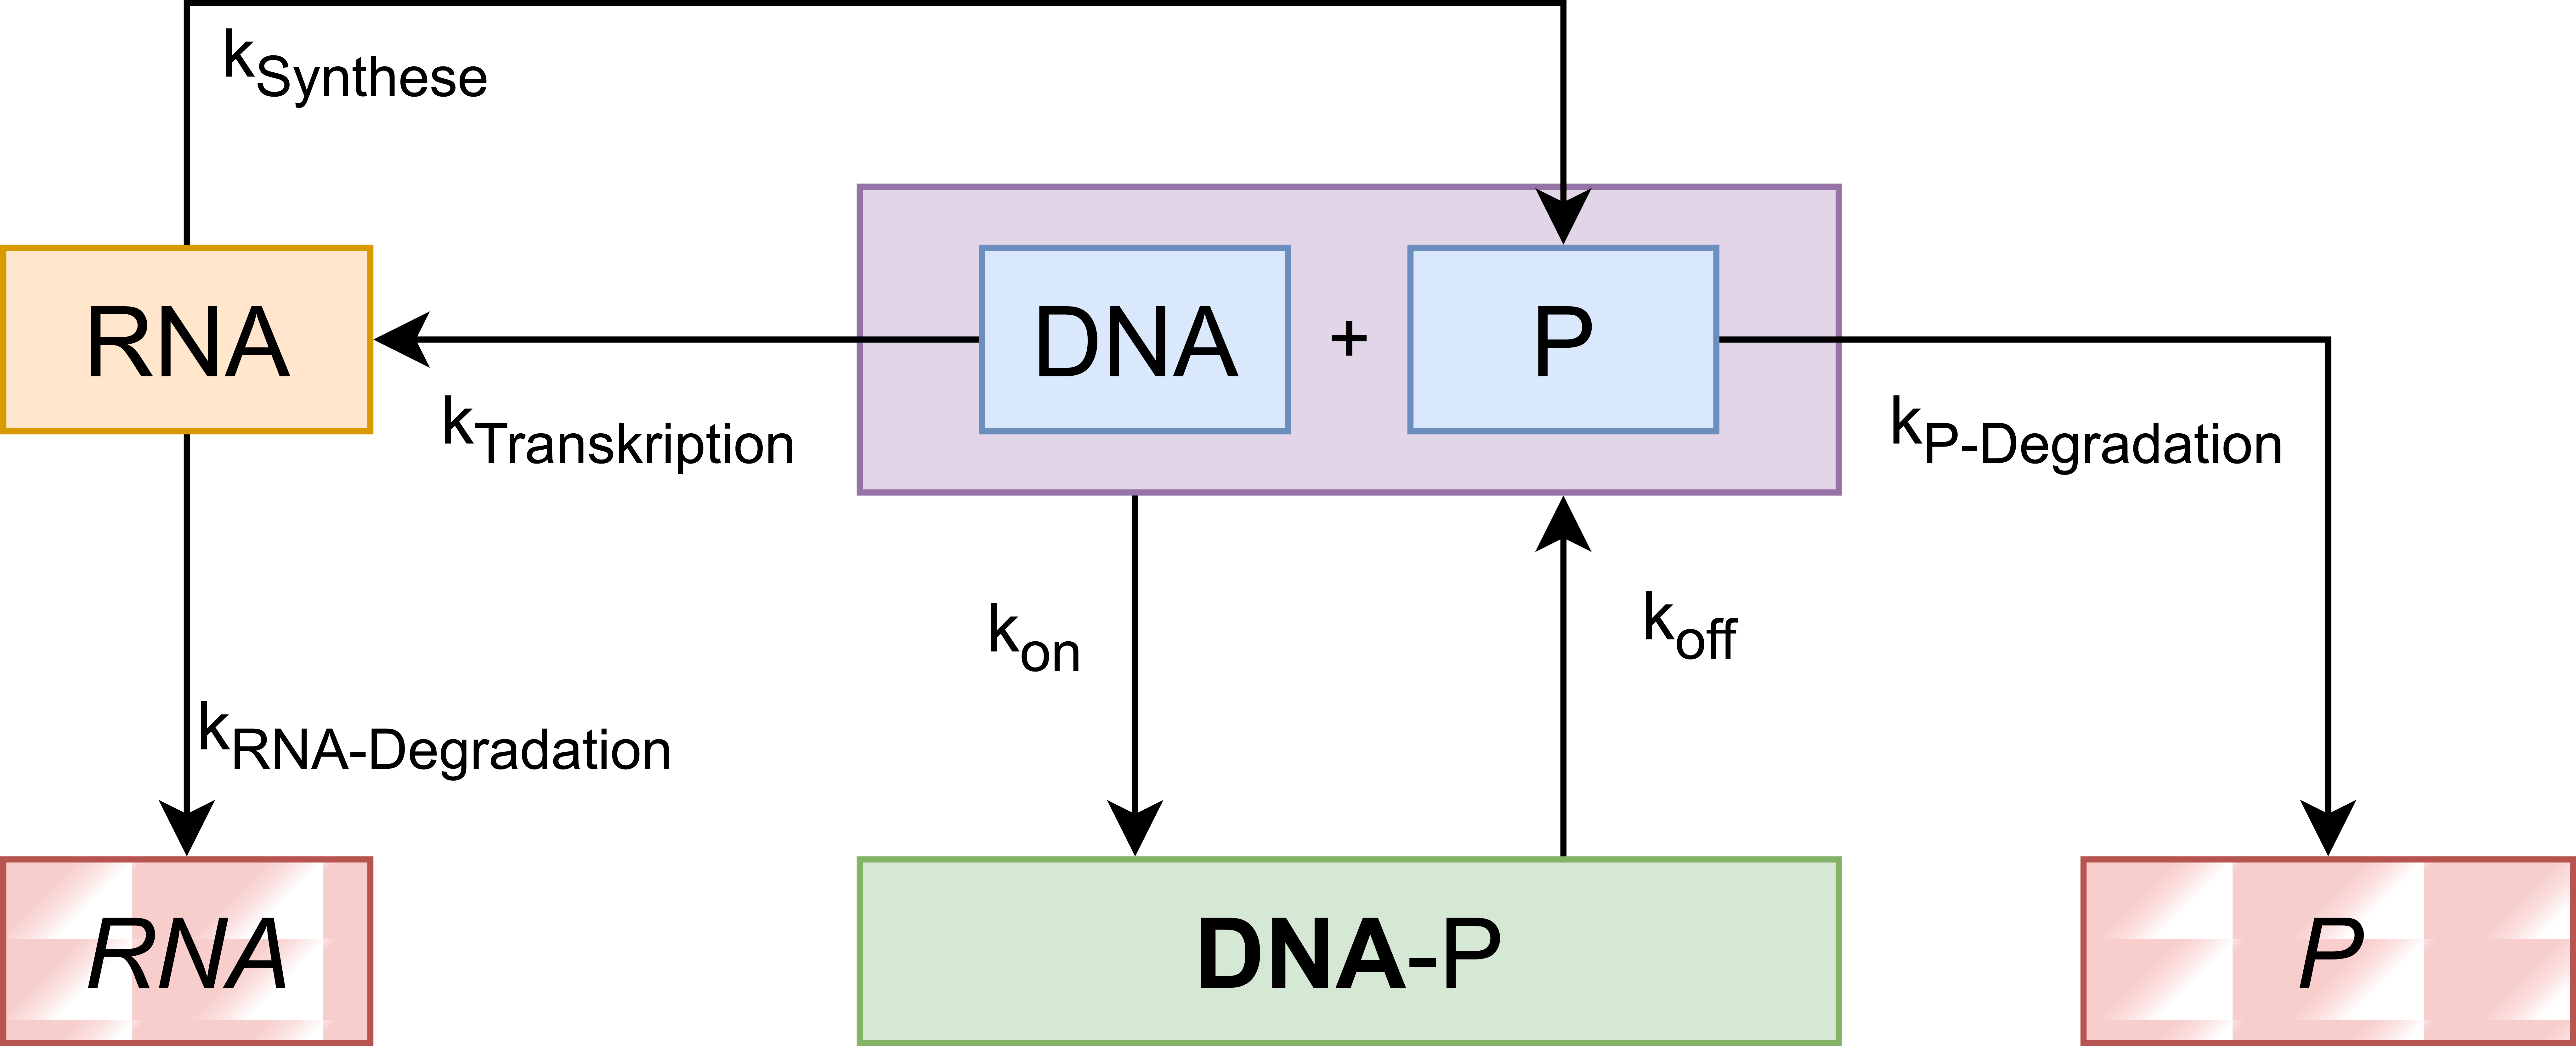
\includegraphics[width=\textwidth]{images/negative_autoregulation_overview.png}

%@Xaver
%\note{Mit Overview neuen Kontext einleiten}
\end{frame}

% Xaver
\begin{frame}{Mathematische Modellierung}
\begin{columns}
    \column{.5\textwidth}
    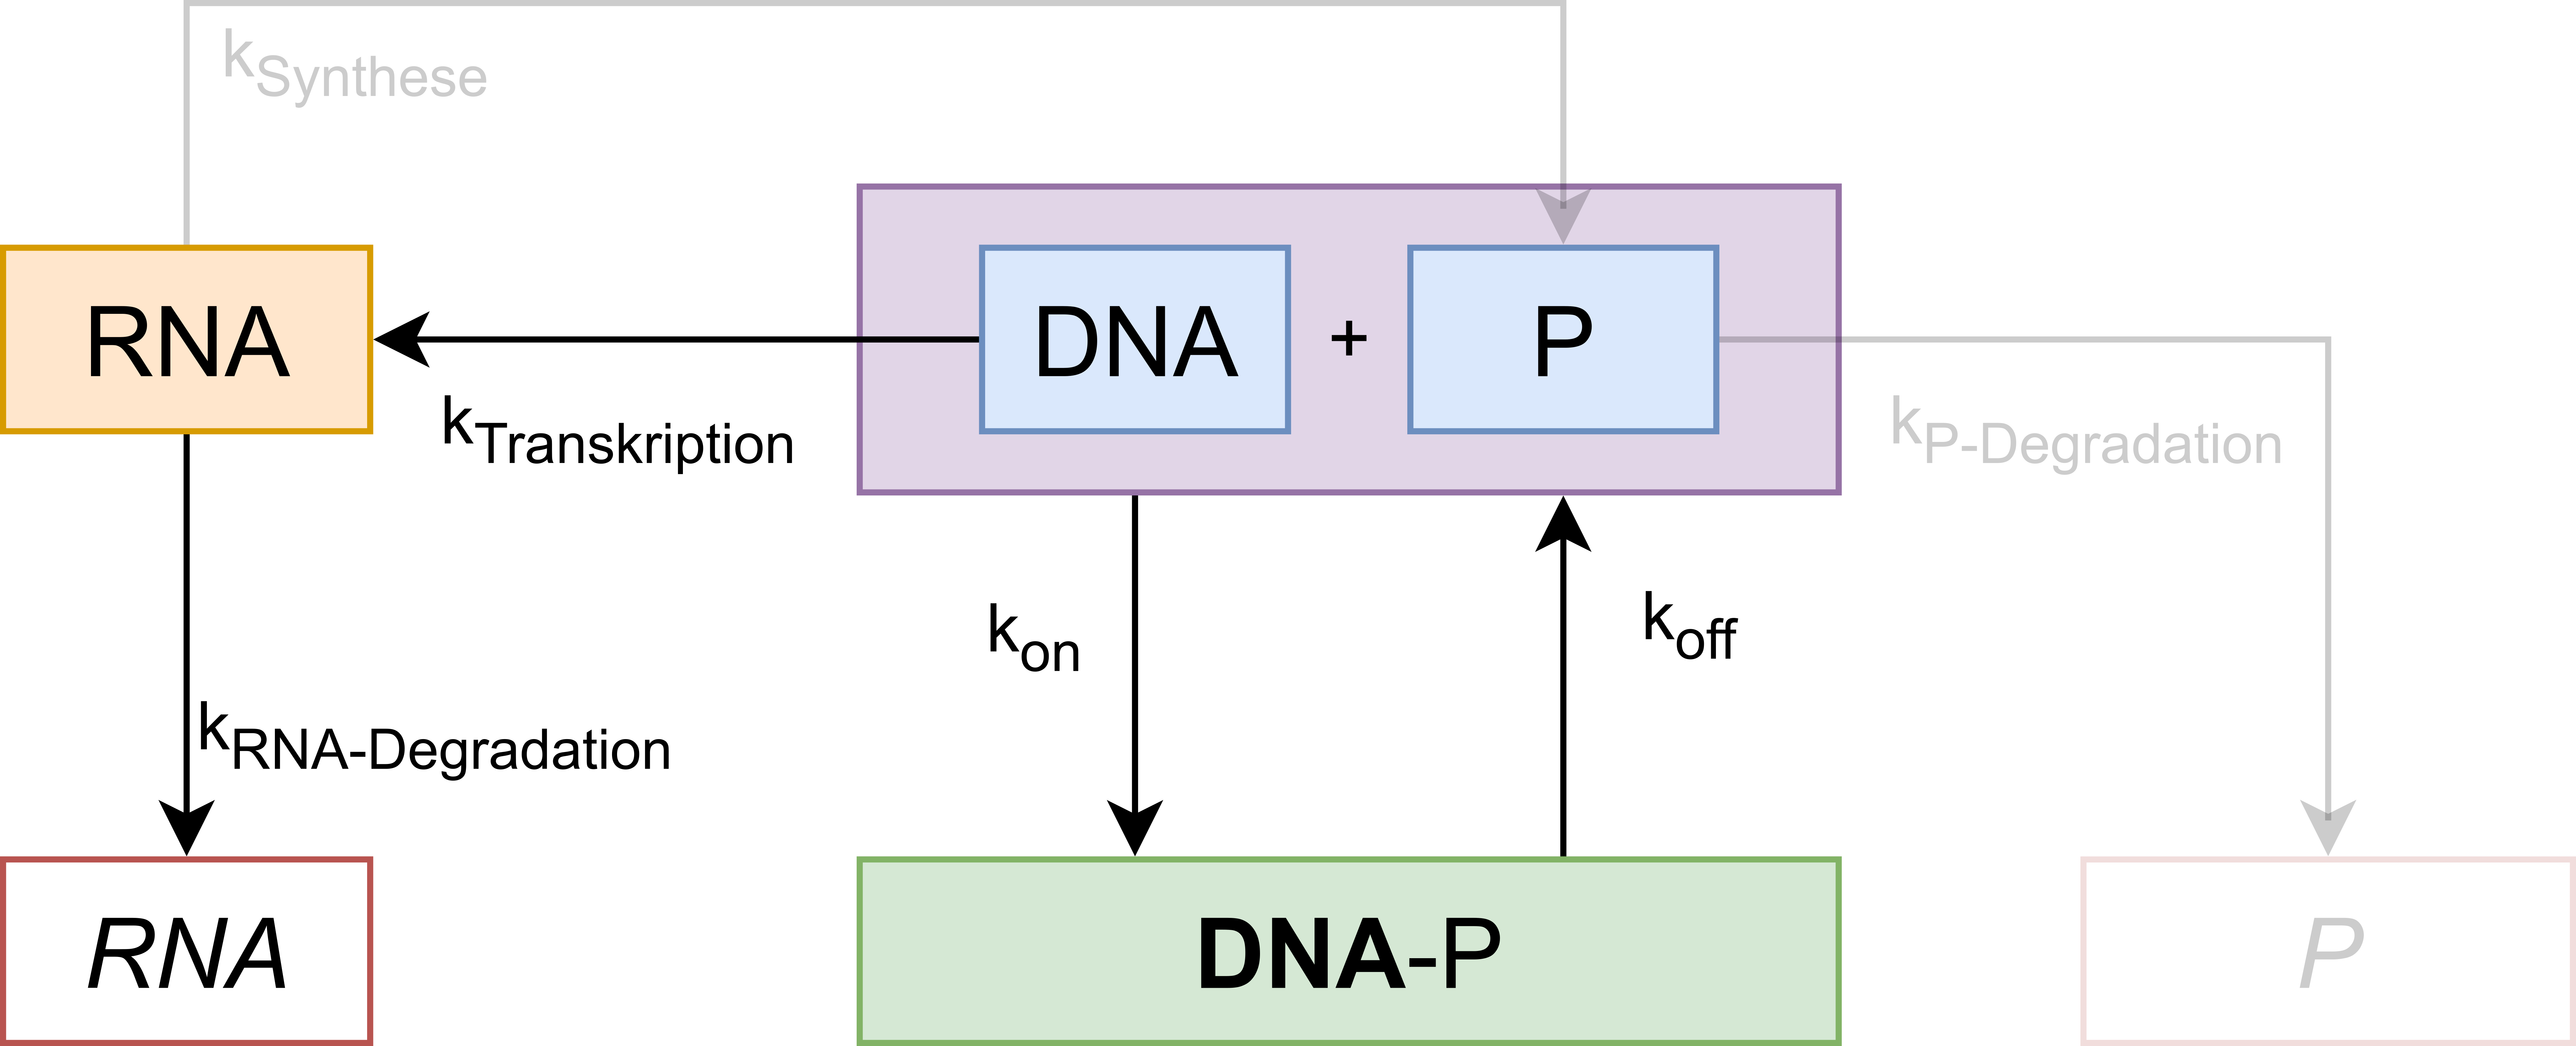
\includegraphics[width=\textwidth]{images/negative_autoregulation_RNA.png}
    \column{.5\textwidth}
    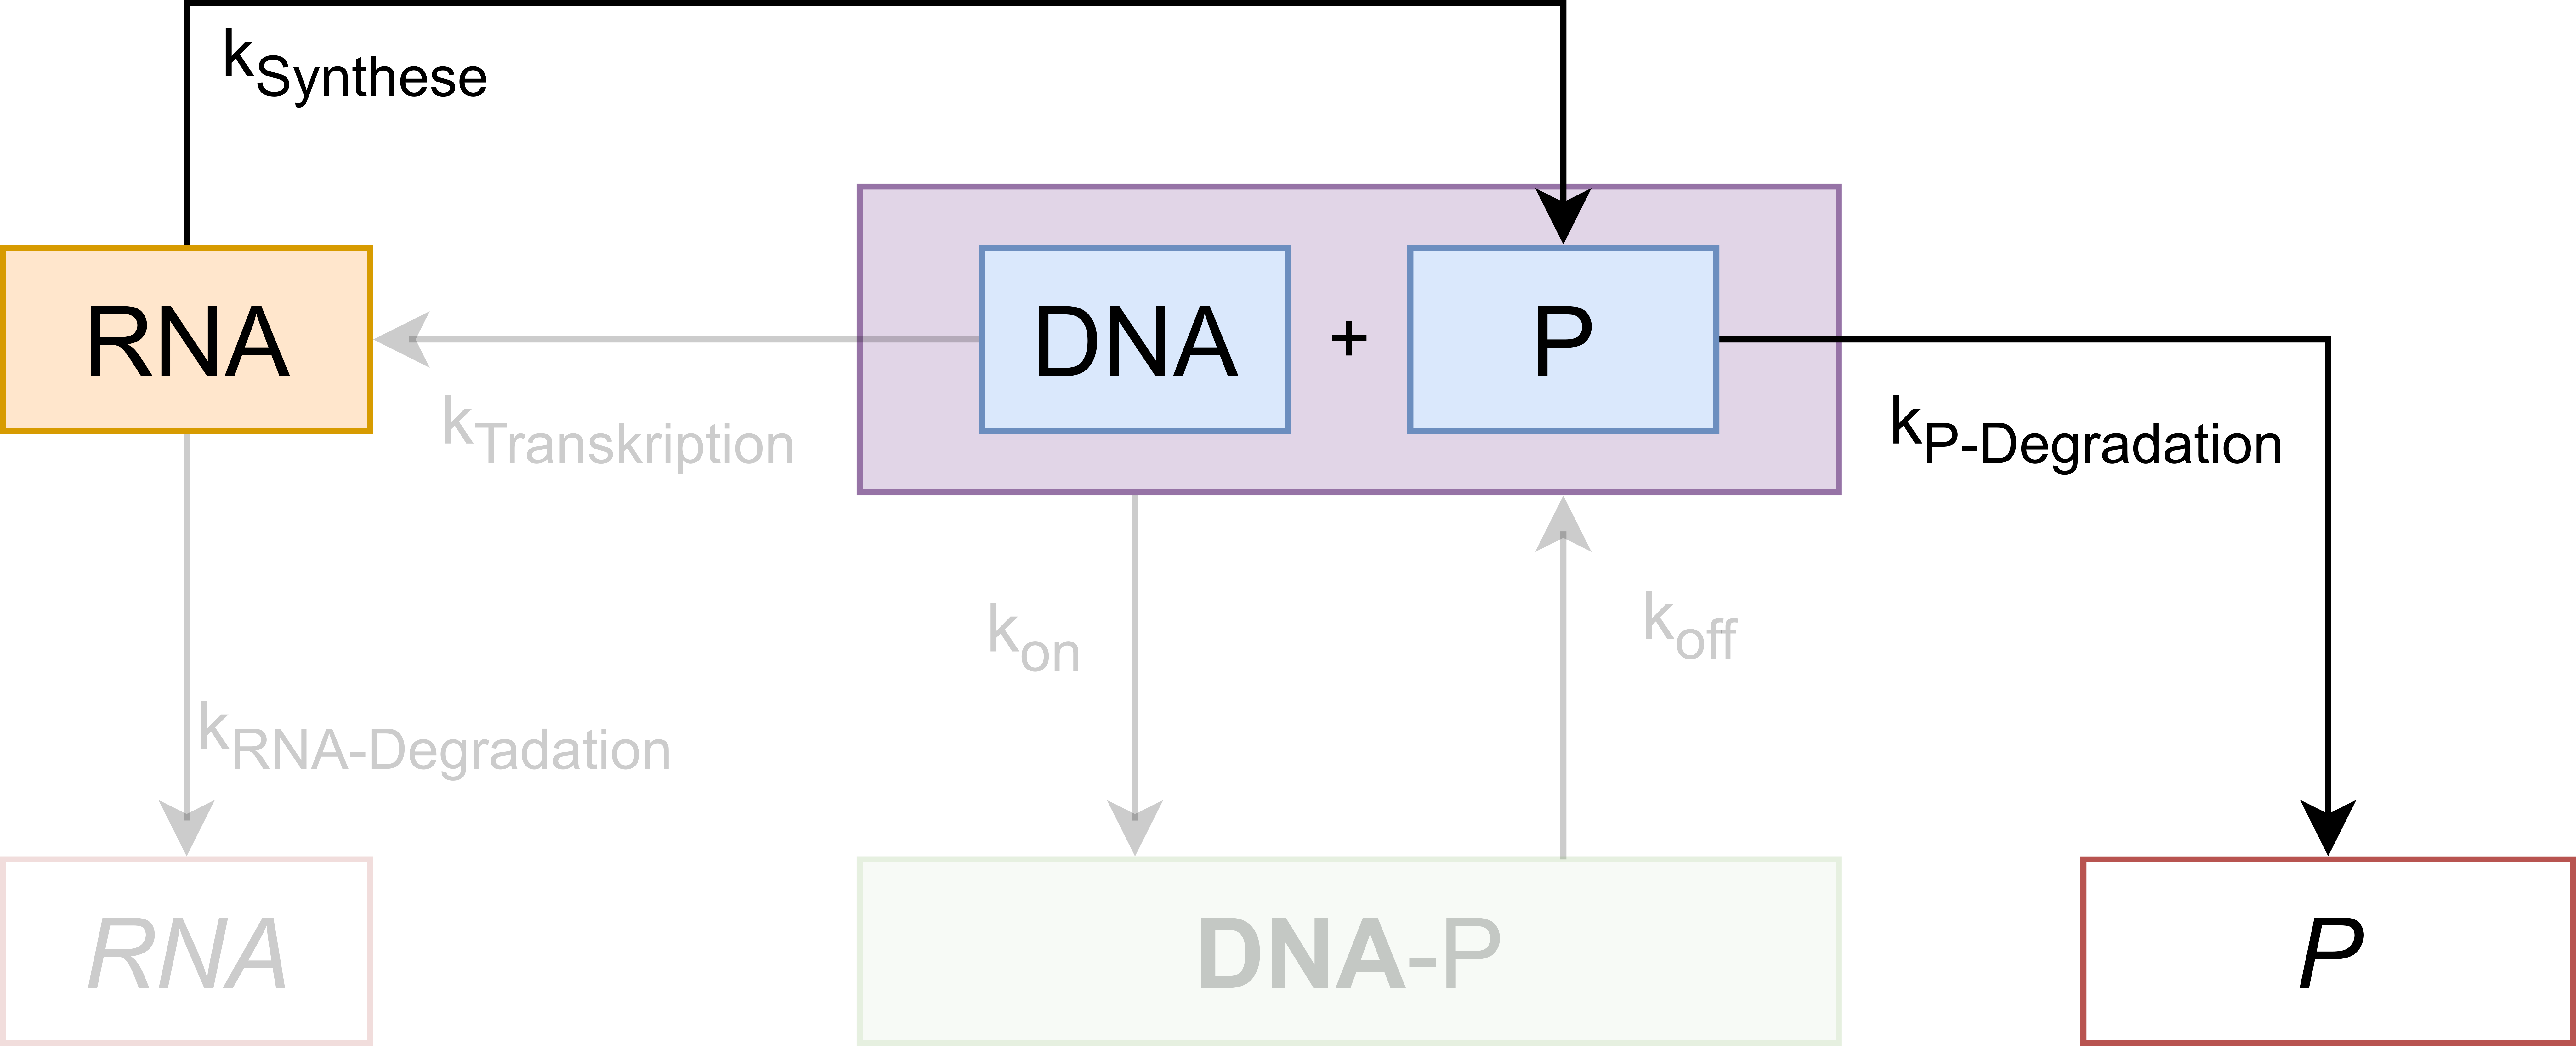
\includegraphics[width=\textwidth]{images/negative_autoregulation_P.png}
\end{columns}
\pause
\vspace{24pt}
\begin{columns}
    \column{.5\textwidth}
    \[\frac{d[\text{RNA}]}{dt}=\text{RNA}_{\text{Synthese}}-\text{RNA}_{\text{Degradation}}\]
    \column{.5\textwidth}
    \[\frac{d[\text{P}]}{dt}=\text{P}_{\text{Synthese}}-\text{P}_{\text{Degradation}}\]
\end{columns}

\end{frame}

% Xaver
\begin{frame}{Mathematische Modellierung mRNA}
    
    \begin{columns}
        \column{0.5\textwidth}
            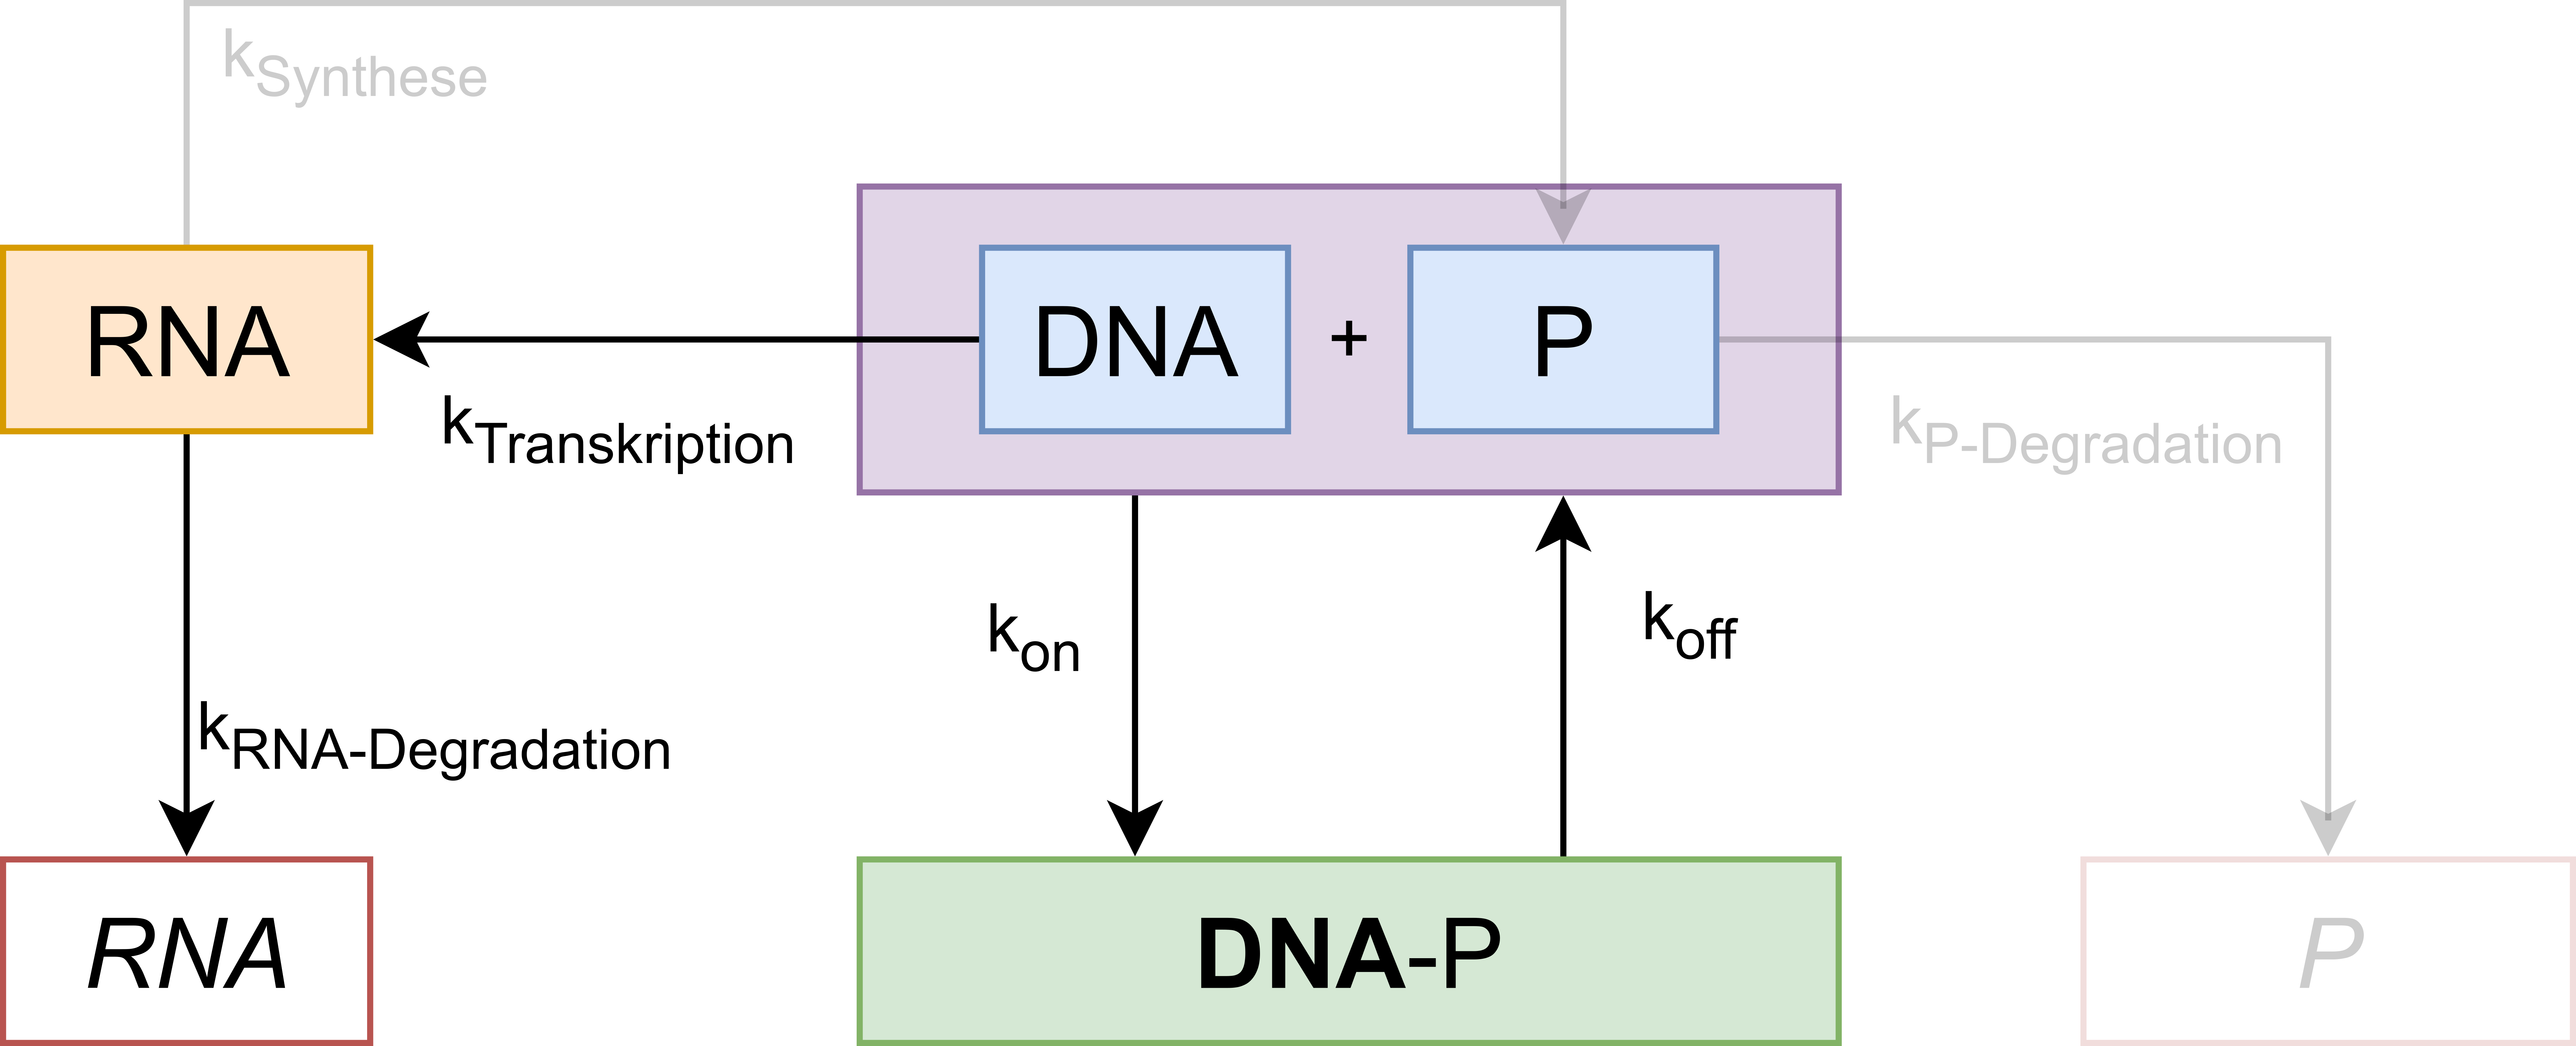
\includegraphics[width=\textwidth]{images/negative_autoregulation_RNA.png}
        \column{0.5\textwidth}

        % pause does not work with the align environment
        \begin{align*}
            \action<+->{\frac{d[\text{RNA}]}{dt}&=\text{RNA}_{\text{Transkription}}-\text{RNA}_{\text{Degradation}}\\[2em]}
            \action<+->{\text{RNA}_{\text{Transkription}}&=}\only<+>{k_\text{t}\cdot [\text{DNA}]}\only<+->{k_{\text{t}} \cdot [\text{DNA}_\text{Total}]  \cdot \frac{K}{K+[\text{P}]}}\\
            \action<+->{\text{RNA}_{\text{Degradation}}&=}\action<+->{k_{dr} \cdot [\text{RNA}]}
        \end{align*}
    \end{columns}

    \vspace{3em}
    \[\action<+->{\frac{d[\text{RNA}]}{dt}=\action<+->{\underbrace{k_{\text{t}} \cdot [\text{DNA}_\text{Total}]}_{v_\text{max}} \cdot \frac{K}{K+[\text{P}]}-k_{dr} \cdot [\text{RNA}]}}\]
\end{frame}

% Mario
\begin{frame}{Mathematische Modellierung Protein}
    \begin{columns}
        \column{0.5\textwidth}
            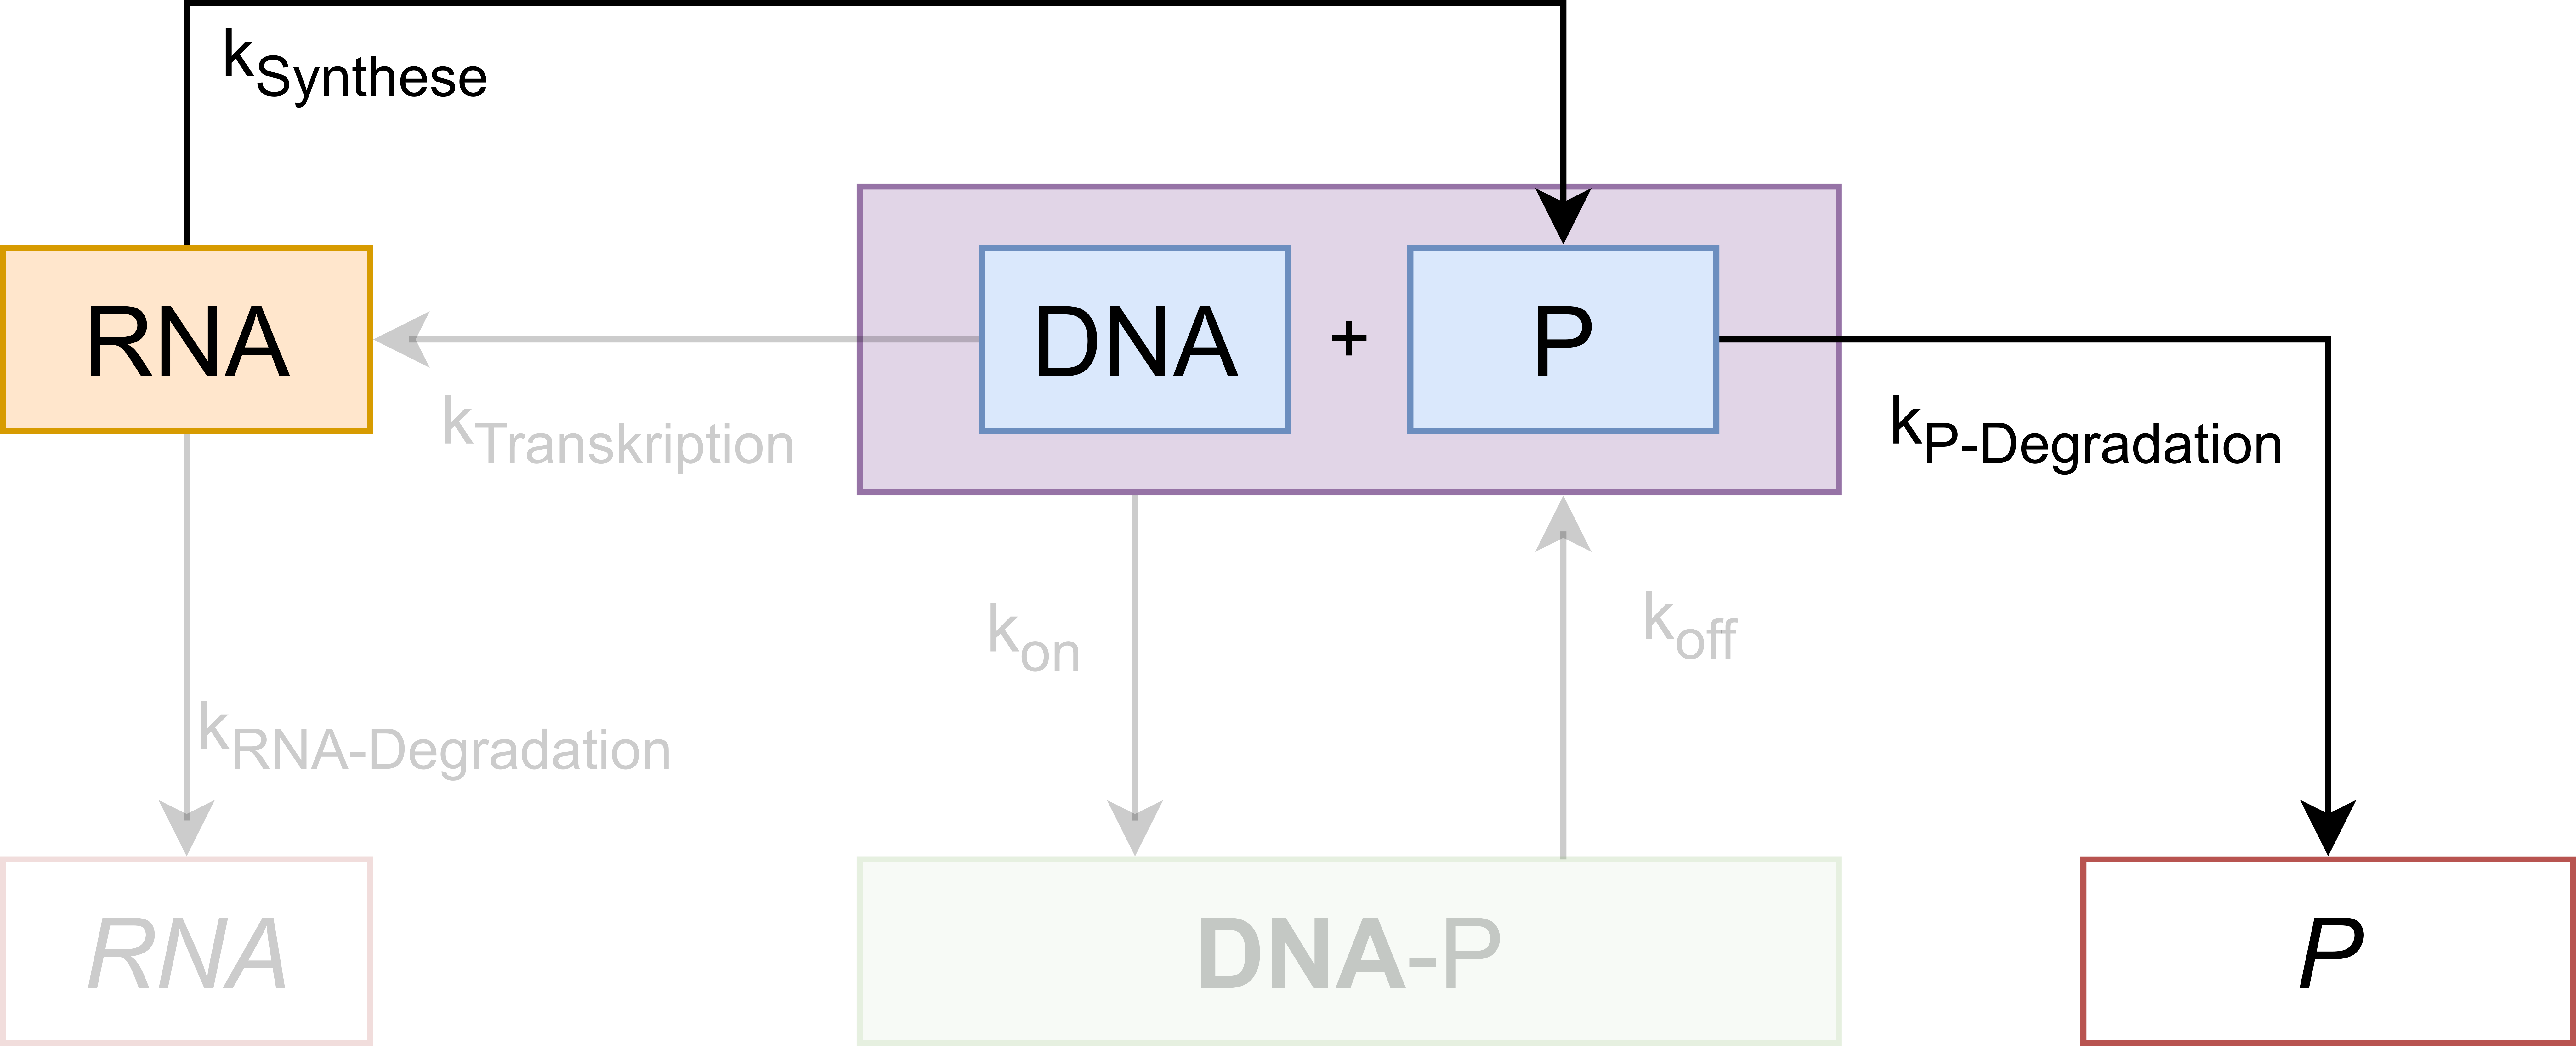
\includegraphics[width=\textwidth]{images/negative_autoregulation_P.png}
        \column{0.5\textwidth}

        \begin{align*}
            \action<+->{\frac{d[\text{P}]}{dt}&=\text{P}_{\text{Synthese}}-\text{P}_{\text{Degradation}}\\[2em]}
            \action<+->{\text{P}_{\text{Synthese}}&=\action<+->{k_s\cdot [\text{RNA}]}\\}
            \action<+->{\text{P}_{\text{Degradation}}&=\action<+->{k_{dp}\cdot [\text{P}]}}
        \end{align*}
    \end{columns}

    \vspace{3em}
    \[\action<+->{\frac{d[\text{P}]}{dt}=\action<+->{k_s\cdot[\text{RNA}]-k_{dp}\cdot[\text{P}]}}\]
\end{frame}

% Mario
\begin{frame}{Mathematische Modellierung}
    \begin{columns}
        \column{.3\textwidth}
        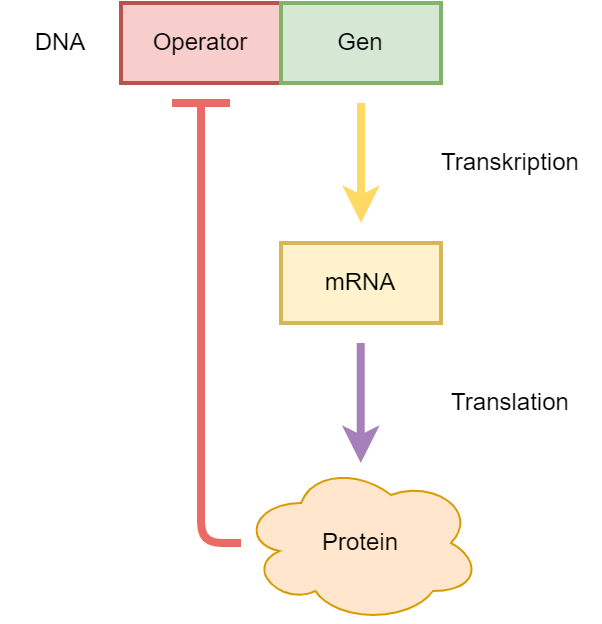
\includegraphics[width=\textwidth]{images/repression.png}
        \column{.7\textwidth}
        \begin{align*}
            \colorbox[HTML]{FFD966}{$\dfrac{d[\text{RNA}]}{dt}$}&=v_{\text{max}}\cdot\frac{K}{K+[\text{P}]}-k_{dr}\cdot [\text{RNA}]\\[16pt]
            \colorbox[HTML]{A680B8}{$\dfrac{d[\text{P}]}{dt}$}&=k_s\cdot[\text{RNA}]-k_{dp}\cdot[\text{P}]
        \end{align*}
    \end{columns}
\end{frame}

% Xaver
\begin{frame}[t]{Stationäre Lösung}

    @Xaver Schnell erklären was eine stationäre Lösung ist und was unser Ziel damit ist

\end{frame}

\begin{frame}[t]{Stationäre Lösung herleiten}
    \begin{columns}[t]
        \column{.5\textwidth}
            \[\frac{d[\text{RNA}]}{dt}=v_{\text{max}}\cdot\frac{K}{K+[\text{P}]}-[\text{RNA}] \cdot k_{dr}\]
        \column{.5\textwidth}
            \[\frac{d[\text{P}]}{dt}= k_s\cdot[\text{RNA}]-k_{dp}\cdot[\text{P}]\]
    \end{columns}
\end{frame}

% Xaver
\begin{frame}[t]{Stationäre Lösung herleiten}
    \begin{columns}[t]
        \column{.5\textwidth}
            \[0=v_{\text{max}}\cdot\frac{K}{K+[\text{P}]}-[\text{RNA}] \cdot k_{dr}\]
        \column{.5\textwidth}
            \[0= k_s\cdot[\text{RNA}]-k_{dp}\cdot[\text{P}]\]
    \end{columns}
    \pause
    \begin{columns}[t]
        \column{.5\textwidth}
            
        \column{.5\textwidth}
            \[\Rightarrow \textcolor{ETHPurple}{[\text{RNA}]}=\frac{k_{dp} \cdot [\text{P}]}{k_s}\]
    \end{columns}
    \pause
    \begin{columns}[t]
        \column{.5\textwidth}
            \[0=v_{\text{max}}\cdot\frac{K}{K+[\text{P}]}-\textcolor{ETHPurple}{[\text{RNA}]} \cdot k_{dr}\]
            \pause
            \[0=v_{\text{max}}\cdot\frac{K}{K+[\text{P}]}-\textcolor{ETHPurple}{\frac{k_{dp} \cdot [\text{P}]}{k_s}} \cdot k_{dr}\]
            \pause
            \[0=[\text{P}]^2 \cdot \underbrace{k_{dp} \cdot k_{dr}}_{a} + [\text{P}] \cdot \underbrace{K \cdot k_{dp} \cdot k_{dr}}_{b} - \underbrace{v_{\text{max}} \cdot K \cdot k_s}_{c}\]
            \pause
            \[[\text{P}] = \texttt{<value>}\]
        \column{.5\textwidth}
            \[\]
    \end{columns}
    \begin{columns}[t]
        \column{.5\textwidth}
            \[\]
        \column{.5\textwidth}
            \[[\text{RNA}] = \frac{k_{dp} \cdot \texttt{<value>}}{k_s}\]
            \[[\text{RNA}] = \texttt{<value 2>}\]
    \end{columns}

\end{frame}

% Xaver
\begin{frame}{Konstanten}
\begin{tabular}{p{.2\linewidth}|p{.4\linewidth}|p{.3\linewidth}}
    Was? & Werte & resultierende Konstante \\ \hline
     Halbwertszeit von bakteriellen Proteinen\cite{Koch1955-sx}\cite{Mandelstam1958-ne}\cite{Maurizi1992} & Wenige Stunden bis zu 70 Stunden bzw. über längere Zeit stabil, je nach Protein und Zustand und Umgebung des Organismus & $k_{dp}=\dfrac{\ln(2)}{60\text{ min}\cdot 15}=0.00077\text{ min}^{-1}$ \\
     Halbwertszeit von mRNA\cite{Bernstein2002-af}\cite{Taniguchi2010-fj}\cite{Selinger2003-or} & Im Bereich von 5 Minuten & $k_{dr}=\dfrac{\ln(2)}{5\text{ min}}=0.138\text{ min}^{-1}$ \\
     Affinität vom TF & Affinität von LacI und DNA & $K=10^{-10}-10^{-11}\text{ M}$ \\
     Average translation rate\cite{Guet2008} & 8 AA/s & $k_s = 3 * 8 = 24 \text{s$^{-1}$}$
\end{tabular}
\end{frame}

\begin{frame}{Numerische Lösungen mit Matlab}
    Simulation des Modells mit bestimmten Anfangswerten
    \begin{itemize}
        \item[$\Rightarrow$] keine Störungen
        \item[$\Rightarrow$] System sollte zu einem Gleichgewicht tendieren
    \end{itemize}

    \vspace{4em}
    \textbf{Was ist Matlab?}\\
    \begin{itemize}
        \item Programmiersprache und -umgebung zum Lösen mathematischer Probleme
        \item \emph{Verfügt über mehrere Funktionen, Differentialgleichungen zu lösen}
        \item Verschiedenste Module unterschiedlicher Anwendungsfelder wie z.B. Computational Biology
    \end{itemize}
\end{frame}

% Mario
\begin{frame}{Numerische Lösung mit Matlab\hfill {\small \color[ETHBblue]{Negative Autoregulation}}}
\begin{figure}
    \centering
    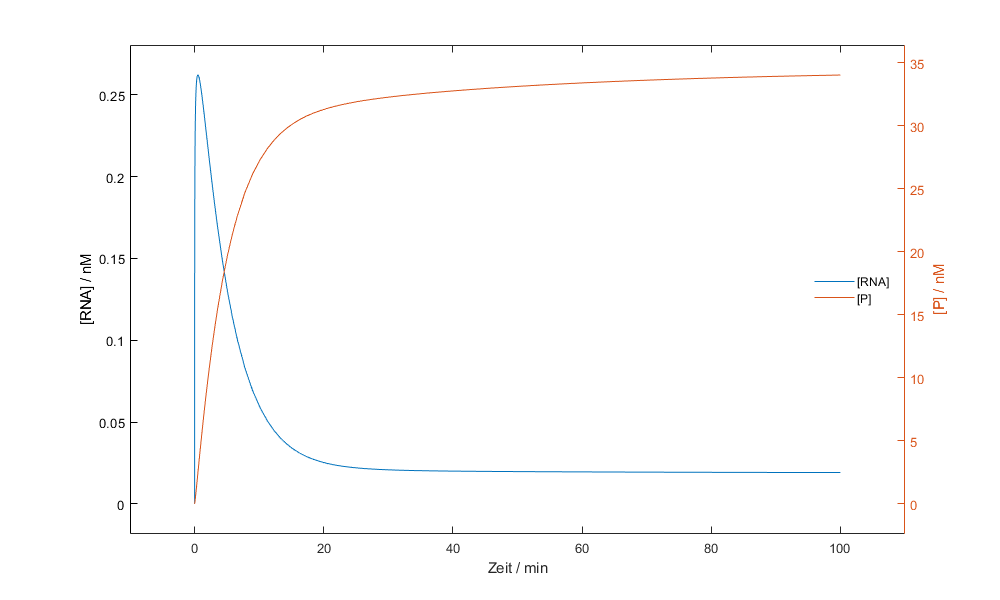
\includegraphics[width=.7\textwidth]{images/simulations/negative_autoregulation_basic.m.png}
\end{figure}
\end{frame}

\begin{frame}{Numerische Lösung mit Matlab\hfill {\small Negative Autoregulation}}
    \begin{columns}
        \column{.4\textwidth}
            \textbf{Gleichgewichtszustand}\\[1em]
            
            \begin{itemize}
                \item $\text{RNA}_\text{Synthese}=\text{RNA}_\text{Degradation}$
                \item $\text{Protein}_\text{Synthese}=\text{Protein}_\text{Degradation}$
                \vspace{1em}
                \item RNA bei ungefähr 0.02 nM
                \begin{itemize}
                    \item \emph{\tiny Vorausgesagt: <stationäre Lösung>}
                \end{itemize}
                \item Protein bei ungefähr 34.5 nM
                \begin{itemize}
                    \item \emph{\tiny Vorausgesagt: <stationäre Lösung>}
                \end{itemize}

                \item $\dfrac{[\text{RNA}]}{[\text{Protein}]}\approx \dfrac{1}{1725}$
            \end{itemize}
        \column{.6\textwidth}
        
        \begin{figure}
            \centering
            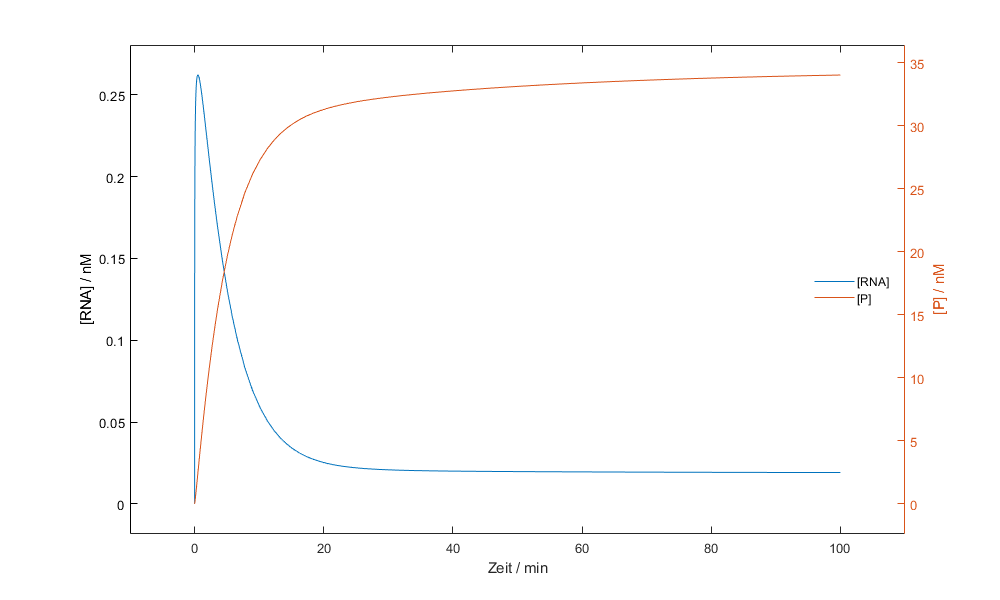
\includegraphics[width=\linewidth]{images/simulations/negative_autoregulation_basic.m.png}
        \end{figure}
    \end{columns}
\end{frame}

\begin{frame}{Unterschiedliche Bedingungen\hfill {\small Negative Autoregulation}}
    \begin{columns}
        \column{.6\textwidth}
        \begin{itemize}
            \item $[\text{P}]_0=0$ eher unwahrscheinlich
            \begin{itemize}
                \item Gleichgewichtszustand wird aber trotzdem immer erreicht
                \item $[\text{P}]_0=38\text{ nM}$
                \item[$\Rightarrow$] RNA geht direkt zum GGW-Zustand, ohne Überschuss
            \end{itemize}
        \end{itemize}
        
        \column{.4\textwidth}
        \begin{figure}
            \centering
            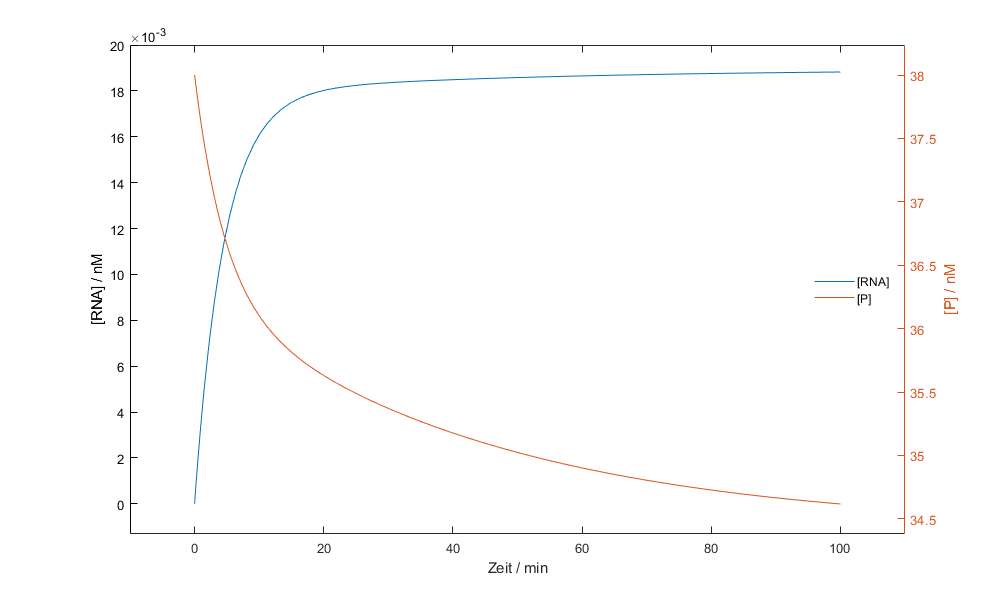
\includegraphics[width=\linewidth]{images/simulations/negative_autoregulation_high_protein.m.png}
        \end{figure}
    \end{columns}
    \pause

    \begin{columns}
        \column{.6\textwidth}
        \begin{itemize}
            \item Affinität des Repressors zur DNA ($K$) hat grossen Einfluss auf die Gleichgewichtskonzentration
            \begin{itemize}
                \item $K=1\text{ nM}$
                \item Je kleiner die Affinität ($\uparrow K$), desto höher die GGW-Konzentration
            \end{itemize}
        \end{itemize}
        \column{.4\textwidth}

        \begin{figure}
            \centering
            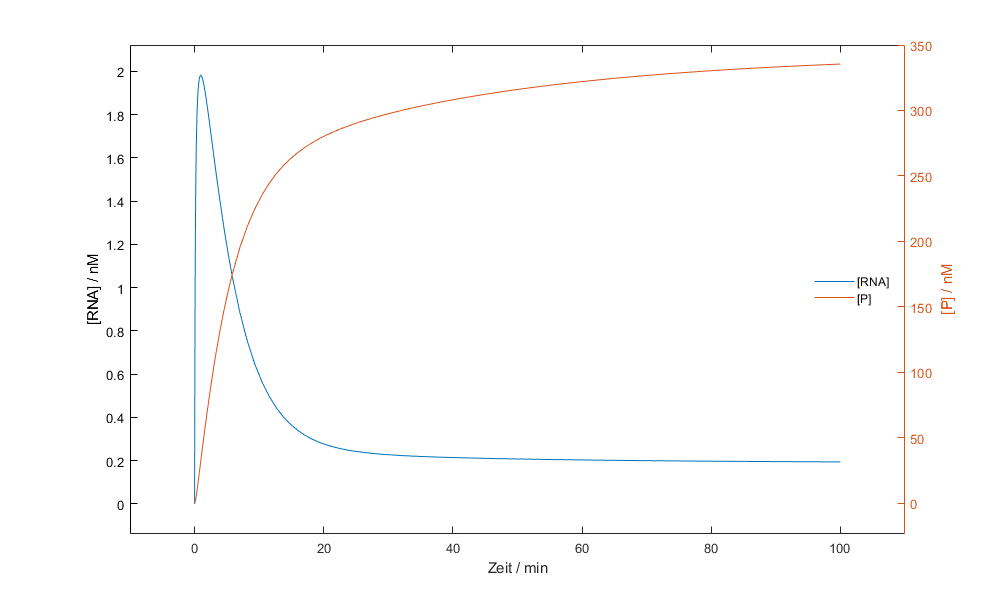
\includegraphics[width=\linewidth]{images/simulations/negative_autoregulation_low_affinity.m.png}
        \end{figure}
    \end{columns}
\end{frame}

\begin{frame}{Unterschiedliche Bedingungen\hfill {\small Negative Autoregulation}}
    \begin{columns}
        \column{.6\textwidth}
        \begin{itemize}
            \item Degradationsraten bestimmen die Zeit bis zum Gleichgewicht
            \begin{itemize}
                \item $k_{dr}=0.46\text{ min$^{-1}$}$
                \item $k_{dp}=0.22\text{ min$^{-1}$}$
                \item Je schneller die Degradation, desto eher stellt sich ein neuer GGW ein
            \end{itemize}
        \end{itemize}
        
        \column{.4\textwidth}
        \begin{figure}
            \centering
            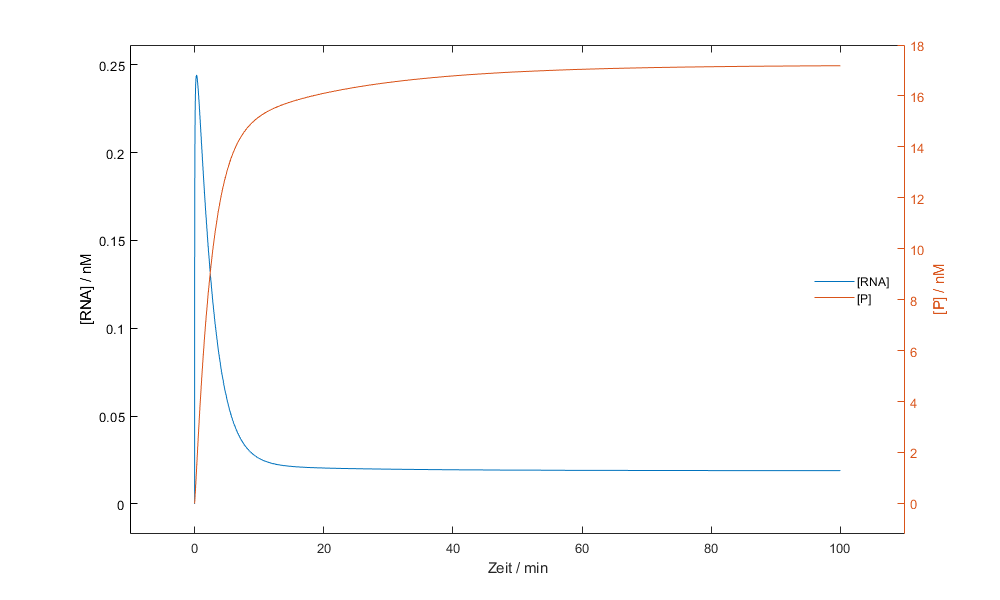
\includegraphics[width=\linewidth]{images/simulations/negative_autoregulation_quicker_degradation.m.png}
        \end{figure}
    \end{columns}
\end{frame}

% Mario
\begin{frame}{Vergleich mit positiver Rückkopplung}
\begin{figure}
    \centering
    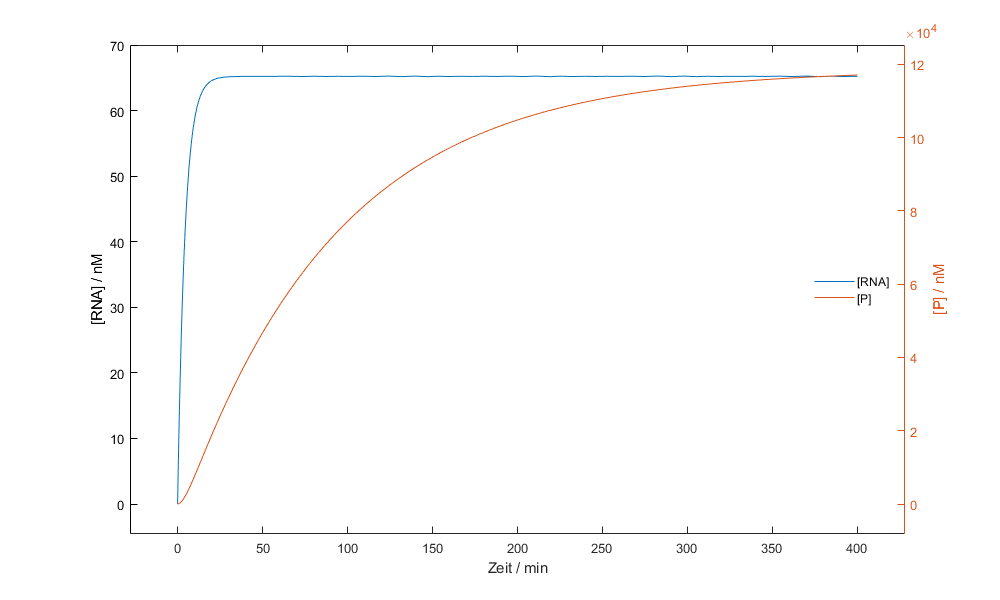
\includegraphics[width=\textwidth]{images/simulations/positive_autoregulation_basic.m.png}
\end{figure}
\end{frame}

% TBD
\begin{frame}{Vereinfachungen}
    \begin{itemize}
        \item Keine Verzögerungen durch Transkription und Translation
        \item Sofortige Einstellung GGW DNA

        % Lac Operon spezifisch
        \item kein CAP $\Rightarrow$ Effekt von Glucose auf die Genexpression
        \item Lactose $\rightleftharpoons$ Allolactose
        \item LacI eigentlich ein Tetramer + kooperative Bindung
        \item Drei Bindungsstellen für Repressor
        \item Lactose-Import in die Zelle durch LacY
    \end{itemize}
\end{frame}

\end{document}